%==================================certificate1.tex================================
% To print name of only the seminar coordinator 1 in the certificate page
\clearpage\thispagestyle{empty}
\subfile{design_cover}
\begin{center}

\leftline{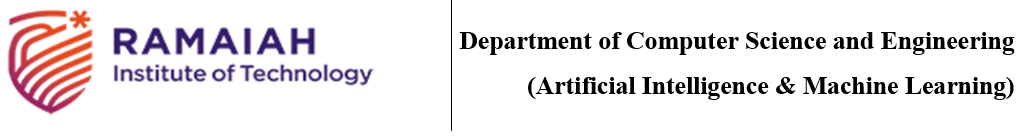
\includegraphics[scale=0.9]{finallogo.PNG}}

\hspace{3.0cm}
\end{center}

\begin{center}
\large\textbf{CERTIFICATE}
\end{center}

Certified that the Mini Project Work (CIP67) entitled "Automated Lifting and Synthesis of Legacy Code into Tensor IR using MLIR" is a bonafide work carried out by Reynesh K (1MS23CI098), Rishab Tarakesh (1MS23CI099), and Yashovardhan Singh Rathore (1MS23CI137), students of M. S. Ramaiah Institute of Technology, Bengaluru, in partial fulfillment of the requirements for the award of Bachelor of Engineering in Computer Science and Engineering (AI\&ML) of Visvesvaraya Technological University, Belagavi during the academic year 2025-26. It is certified that all corrections and suggestions indicated during internal assessment have been incorporated, and the report satisfies the prescribed academic requirements for Mini Project Work.

\vspace{1 cm}
\begin{center}

\begin{table}[ht]
\centering
\begin{tabular}{p{5.0cm} p{5.0cm} p{5.0cm}}
Signature of Guide 1 & Signature of Guide 2 & Signature of HoD \\
\textbf{Dr. Mohana Kumara S} & \textbf{Dr. Sini Anna Alex} & \textbf{Dr. Siddesh G M} \\
Associate Professor (CSE(AI\&ML)) & Associate Professor (CSE(AI\&ML)) & Professor \& Head \\
Dept. of CSE(AI\&ML) & Dept. of CSE(AI\&ML) & Dept. of CSE(AI\&ML) and Dept. of CSE(CS)\\
\end{tabular}

\end{table}
\end{center}

External Examiners\\
The external examiners will be nominated by the university at the time of final viva-voce evaluation.
\thispagestyle{empty}
